\documentclass[9pt,twocolumn,twoside]{article}
% Use the lineno option to display guide line numbers if required.
% Note that the use of elements such as single-column equations
% may affect the guide line number alignment.

\usepackage{amsmath}
\usepackage{graphicx}
\usepackage{subcaption}
\usepackage{breqn}
\usepackage{color}

\newcommand\davidsays[1]{{\em\color{blue} {\bf DR:} #1}}

% the follow ing causes latex to not wait interactively
% \nonstopmode

\captionsetup[subfigure]{singlelinecheck=off,justification=raggedright, margin=0pt, parskip=0pt, skip=0pt}

\title{Brownian dynamics simulation of cytoplasmic dynein's powerstroke reproduces bidirectional stepping}

\input{../../data/paper_params.tex}

\begin{document}
\maketitle

\begin{abstract}
  Please provide an abstract of no more than 250 words in a single paragraph. Abstracts should explain to the general reader the major contributions of the article. References in the abstract must be cited in full within the abstract itself and cited in the text.
\end{abstract}

%\section*{TODO August 2020}
%\begin{enumerate}
%  \item Get new simulations working !!!!!!!!!!!!!!!!!!!
%  \item Articulate data we fit to
%  \begin{enumerate}
%    \item Velocity -> unbinding rate
%    \item Ratio of leading vs trailing steps -> exponential parameter
%    \item Average step length -> other parameters
%    \item Yildiz weird slope -> sticky rate + binding rate
%    \item Avoid instant rebinds -> sticky rate
%    \item Time to kick from MD??
%    \item efficiency (affects instant rebind)
%  \end{enumerate}
%  \item Do the fit (requires 1 above)
%  \item Could have a fixed binding immunity time rather than sticky rate
%  \paragraph{Advantages of immunity time}
%  \begin{enumerate}
%    \item Might accurately reflect a diffusive escape from an energy well
%  \end{enumerate}
%  \paragraph{Advantages of sticky rate}
%  \begin{enumerate}
%    \item Accurately reflects the dynamics of a chemical process
%  \end{enumerate}
%\end{enumerate}


\newpage

%% \dropcap{C}ytoplasmic dynein-1 is a motor protein used to generate directed force in cells. The protein is a homodimer which binds to cellular filaments known as microtubules (MTs). Each monomer has several ATPase domains arranged in a larger globular domain known as the ``head''. This head is the site which hydrolyzes ATP and undergoes the conformational changes responsible for dynein's step. The head is attached via a long chain to the microtubule binding domain (MTBD). Dynein is an interesting structure in that it manages to coordinate ATPase chemistry at its head with MT-releasing chemistry at its MTBD, some 20nm away \cite{mt-atp-coupling}. The head has a long tail domain coming off it, which eventually dimerizes to the other monomer.\\

%% Dynein is unique in that it has a widely varied step size. Dynein's average step is 8 \textit{nm} in the forwards direction, but it is capable of taking 32 \textit{nm} steps in the forwards and reverse directions \cite{weihongpaper} \cite{yildizpaper}. This stochastic, varied stepping is contrasted with the much more regular 8 \textit{nm} step size of kinesin, another bipedal motor protein \cite{kinesin-step-size}. It has been suggested that the long separation between dynein's MTBD and dimerization sites facilitates larger diffusive searches, allowing dynein to take larger steps than kinesin \cite{cargotransport}.\\

%% A simple explanation for dynein's stepping pattern can be given based on only a few facts about the protein. It is known that on treatment with ATP, the tail-head-MTBD angle of a dynein monomer alters, moving the MTBD closer to the tail \cite{carteradpprimed} \cite{burgess-paper}. It is also known that the nucleotide state of the head communicates with the MTBD. ATP binding at a head ATPase shifts the MTBD from a strong to weak MT-bound state. And vice-versa, whether the MTBD is bound or unbound from the MT changes the ATPase rate at the head. From this it is possible to infer a simple model for the dynein stepping cycle. This model, known as the mechanochemical cycle \cite{cianfroccoreview}, has dynein unbind MT, kick forward, diffuse to the next MT binding site, rebind MT, then repeat. Whether a model this simple can explain dynein's behavior needs to be tested.\\

%% Several computational models have been created to explain dynein's motility. \textit{Imamula et. al.} define a chemical transition model which defines all the MT- and nucleotide-bound states dynein goes through as it walks \cite{imamulamodel}. \textit{Sarlah et. al} simulate a model obeying rate constants from \textit{Imamula}, and replicate dynein's stepping trajectory \cite{sarlahmodel}. \textit{Zheng} uses normal mode analysis to simulate the dynein motor's transition from pre to post-stroke \cite{normalmodes}. To our knowledge, no computational model exists which takes into account the microscopic dynamics of protein-water interactions to test whether diffusion is enough for dynein motility. Here we show how a simple Brownian dynamics model can be used to test the mechanochemical cycle picture of dynein processivity.\\


%% Dynein has several cofactors which alter its dynamics. For example, the motor's stall force is tripled when exposed to dynactin and Bic2D \cite{yildizdynactin}. This is odd, since the dynactin- and Bic2D-binding site on dynein is on the tail, far from the motor heads.

Dynein is a motor protein which generates motion for various cellular processes. Cytoplasmic dynein-1, here referred to as ``dynein,'' is a motor which performs cargo transport and aids in nuclear division. The protein consists of a ring structure of six AAA+ domains known as the ``head'' which connect via a long stalk to a microtubule binding domain (MTBD). The AAA+ region is responsible for hydrolyzing ATP to drive dynein's motion. The head is connected via a linker to a large tail domain responsible for binding various cargos and accessory proteins. The tail is also the site of dimerization, where two dynein monomers join to form a homodimeric unit capable of motion.

Dynein's mechanism of motion generation is the least understood of all motor proteins \cite{}. Kinesin and myosin both take consistent steps of the same size \cite{kinesin-step-size, myosin-step-size, is-this-true-in-general-i-thought-only-types-of-myosin}. In contrast, dynein is known to take highly variant steps both forwards and backwards, averaging 16nm \cite{yildizpaper, weihongpaper}. Another interesting feature of dynein is the 20nm separation between its ATP hydrolysis and the site and MT binding site \cite{3vkh-cite}. The protein must transmit information about ATP binding across this distance in order to coordinate its steps \cite{mt-atp-coupling}. Explaining these phenomena is necessary to fully understand dynein's mechanism.

Studies over the past 15 years have shed much light on dynein's stepping mechanism. The motor is known to switch between two conformational states depending on its ATP hydrolysis state \cite{burgess-paper, FRETstatepaper, carter-paper, nicastro, schmidt-carter}. It is also known that ATP binding can induce structural changes within the motor which increase unbinding rate \cite{leschziner, carter-paper}, and similarly that microtubule rebinding can influence nucleotide unbinding rate \cite{mt-atp-coupling}. Taken together this evidence is synthesized into a mechanochemical cycle \cite{cianfroccoreview, imamulamodel, tsygankovscheme}. In this scheme, dynein binds ATP, causing structural changes which eventually lead to microtubule unbinding at its MTBD. These structural changes transition the motor into a more open position, causing the MTBD to diffuse forwards on the microtubule. This biased search is known as the prestroke. Eventually the MTBD rebinds the microtubule, causing structural changes inducing the ejection of hydrolyzed ADP and transitioning back to the closed position. This puts the motor in the post-stroke state, moved forward slightly. The protein is now ready to re-bind ATP and take another step.

This mechanochemical cycle of chemical transitions is well supported by evidence \cite{citemore}. However, there is still relatively little known about the dynamic mechanism of domain motion dynein uses to achieve its forward motion by transitioning between these states \cite{lippert}. There exist models theorizing how dynein's domains move during its forward step, such as the winch \cite{} and powerstroke \cite{} models, which can reproduce experimental data \cite{}. However, to our knowledge, no studies exist which use protein dynamics to study if either of these dynamic mechanisms is feasible for the dynein motor to produce. Existing computational models of walking use chemical rate transitions and assume independence of steps, without simulating the precise protein dynamics \cite{}. Molecular dynamics simulations exist, but are of too short a timescale to describe dynein's forward stroke \cite{}. It is necessary to model dynein dynamically at a large timescale using physically realistic protein dynamics to fully understand how feasible models like the winch and powerstroke are. Further, such long-timescale dynamic models could be used to find what elements of dynein are sufficient to produce forward motion. Further, an accurate dynamical model would allow us to test if certain dynamical elements, such as electrostatic interactions with the microtubule \cite{longrangemt}, ring stacking \cite{sarlahmodel}, discrete microtubule binding sites \cite{trottmodel}, or elasticity of the stalk \cite{burgess-paper} are necessary for dynein's walk.

Here we use a Monte Carlo simulation that investigates dynein's inter-step correlations as it moves along the MT. We model cytoplasmic dynein by reducing the mechanochemical cycle into two states: the pre-stroke and post-stroke states. We use cryo-EM data to create rough structural models of these conformers, and impose inter-domain tension and elastic restoring forces to describe the dynamics within each conformer. We then model the state transition as a transition between two equilibria, and use Brownian dynamics to simulate the model's behavior in physically realistic drag and diffusion conditions. This minimal model spontaneously generates a powerstroke-like dynamic mechanism, and uses it to produce bidirectional motion. The model also reproduces several experimental measures, such as step length and the probability of stepping. 
%% velocity and force-mediated directionality control.

\begin{figure}[tbhp]
\centering
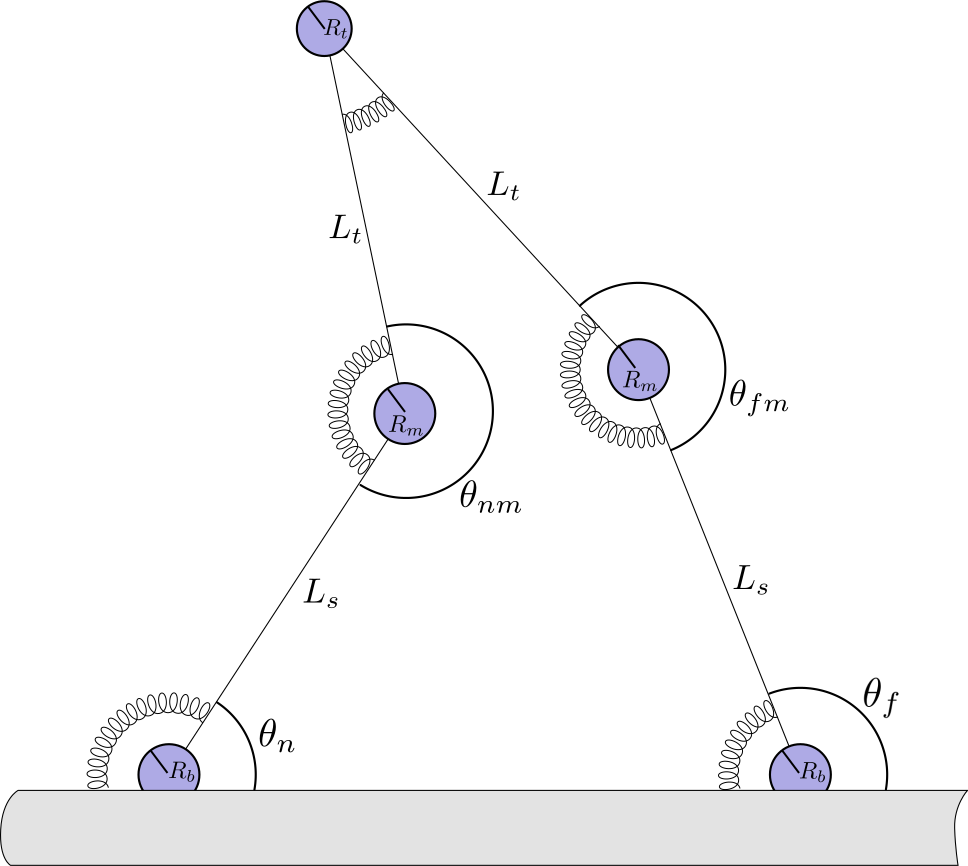
\includegraphics[width=\linewidth]{figures/model-cartoon-simple.pdf}
\caption{\textbf{Basic geometric model in pre-stroke and post-stroke states.} \textit{Left: } Pre-stroke model of dynein with one MTBD bound to microtubule and the other free. Angles are measured from the $+\hat{x}$ direction. \textit{Right: } Post-stroke model with both MTBDs bound to microtubule. MTBD angles are relative to $+\hat{x}$ direction, and motor angles are between stalk and tail. Lengths and radii not to scale.}
\label{fig:model}
\end{figure}

\begin{figure}[tbhp]
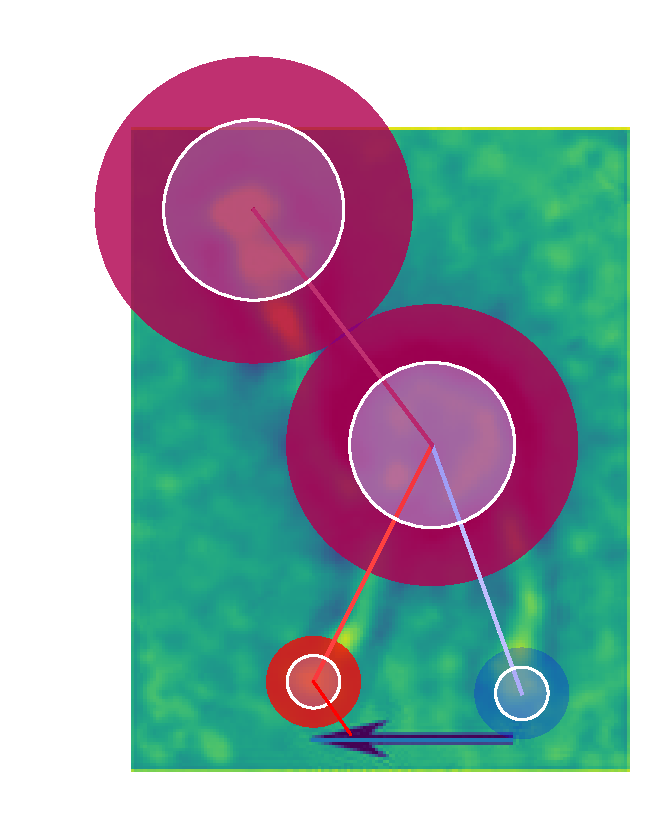
\includegraphics[width=0.4\linewidth]{../../plots/burgess-model-figure.pdf}%
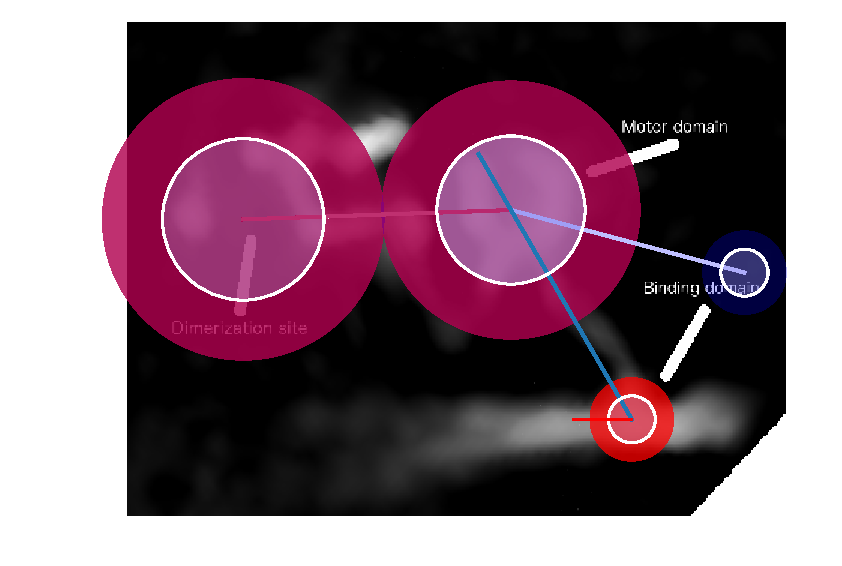
\includegraphics[width=0.6\linewidth]{../../plots/grotjahn-model-figure.pdf}%
%% 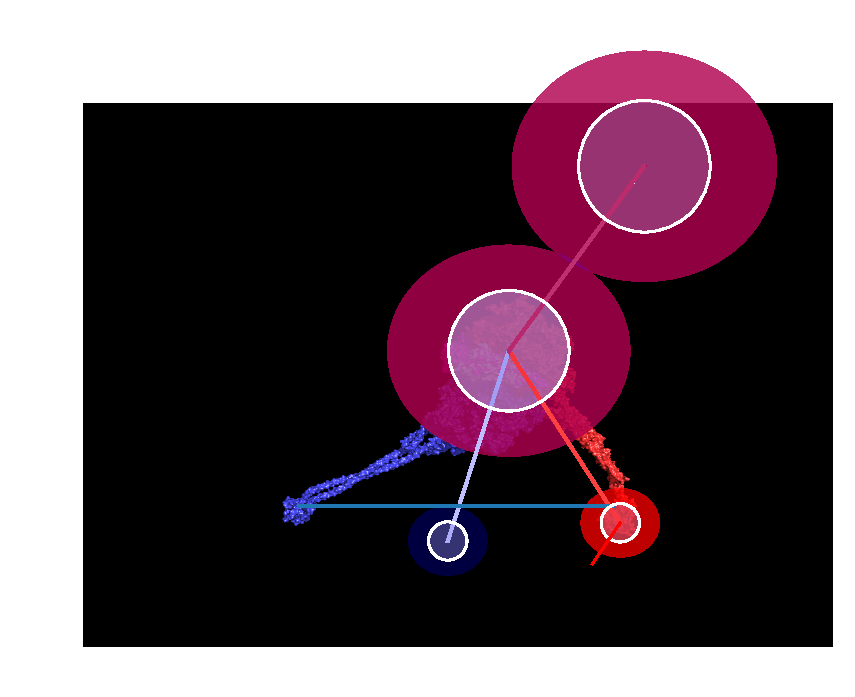
\includegraphics[width=0.3\linewidth]{../../plots/crystal-model-figure.pdf}%
\caption{\textbf{Scale model compared with experimental images.} \textit{Left:} Model with angles at pre-stroke equilibrium superimposed over axonemal dynein c heavy chain micrograph in the pre-stroke ADP-Vi-bound state \cite{burgess-paper}. Interdomain lengths and radii scaled to micrograph scale bar. No microtubule is present, so $\theta_{nb}$ is arbitrary. \textit{Right: } Model with angles at pre-stroke equilibrium superimposed over density map of full-length native cytoplasmic dynein with accessory tail proteins (map ID EMD-7000) \cite{grotjahn}. Interdomain lengths and radii scaled to density map.}
\label{fig:micrographs}
\end{figure}


%% Model at equilibrium angles superimposed over an axonemal dynein c micrograph consisting of an apo and and ADP-Pi-bound dynein monomer \cite{burgess-paper}; axonemal and cytoplasmic dynein have comparable size and architecture \cite{dynein-c-paper}. \textit{Right:} Model at equilibrium superimposed over full-length dimerized dynein bound to accessory proteins,  Left figure has a scale bar of 15nm, right 26.3nm between MTBD and AAA1 of motor domain.


\begin{table}
  \centering
  \begin{tabular}{lrrr}
    Param & Model & Experimental & Source \\
    \hline
    $c_b$ & $\cb \Delta G_{ATP}$ &  & \\
    $c_m$ & $\cm \Delta G_{ATP}$ &  & \\
    $c_t$ & $\ct \Delta G_{ATP}$ &  & \\
    $k_a$ & $\kstk$  $s^{-1}$ &  & \\
    $k_b$ & $\kb$  nm $s^{-1}$ &  & \\
    $\epsilon$ &  $\MTbindingdistance$ nm & & \\
    $k_{ub}$ & $\kub$ $s^{-1}$ & & \\
    $C$ & $\cexp$ & & \\
    $L_s$ & $\ls$ nm & $21$ nm & \cite{Burgess2003, 3vkh-cite, carter-paper}\\
    $L_t$ & $\lt$ nm & $23$ nm & \cite{Burgess2003, 3vkh-cite, carter-paper}\\
    $\theta_b$ & $\eqb$ &  120 & \cite{leschziner} \\
    $\theta_m^{\mbox{pre}}$ & $\eqmpre$ &  197 & \cite{Burgess2003}\\
    $\theta_m^{\mbox{post}}$ & $\eqmpost$ & 242 & \cite{Burgess2003}\\
    $\theta_t$ & $\eqt$ &  & \\
    $R_t$ & $\radiust$ nm & $4$ nm & \cite{Burgess2003}\\
    $R_m$ & $\radiusm$ nm & $5.5$ nm & \cite{Burgess2003}\\
    $R_b$ & $\radiusb$ nm & $1.25$ nm & \cite{Burgess2003}\\
    \hline
  \end{tabular}
  \caption{Parameters used in simulation. $c_b$, $c_m$ and $c_t$ are the MTBD, motor and tail spring constants, respectively. $k_b$ and $k_{ub}$ are the rates of pre-stroke to post-stroke and post-stroke to pre-stroke transitions, respectively. $L_s$ and $L_t$ are the lengths of the stalk and tail interdomain linkers. $c$ is the tension-gating factor. The $\theta$ values are the equilibrium values for each angle, where $\theta_m^{\mbox{pre}}$ is the equilibrium angle for the unbound motor in pre-stroke, whereas $\theta_m^{\mbox{post}}$ is the equilibrium angle for the bound pre-stroke motor and both post-stroke motors. $R_b$, $R_m$ and $R_t$ are the MTBD, motor and tail radii. Parameters used for all simulations unless otherwise noted}
  \label{table:params}
\end{table}

\section{Model}
This model is meant to capture the coarse-grained structural, dynamical and chemical properties of the full dynein complex, while remaining mathematically simple. The structural features of dynein are captured through a two-dimensional geometric model of circular domains connected by rigid rods, shown in Figure \ref{fig:model}. The dynamics of dynein are simulated by imposing both equilibrium and Brownian forces on each circular domain of the model. The chemical properties of dynein are emulated by sporadically transitioning the model between two states: a poststroke state where both binding domains are fixed to the microtubule, and a prestroke state where one foot is free to diffuse. This was influenced by similar simulations done before \cite{zhaomodel}. The poststroke state is meant to represent dynein after rebinding free MTBD and undergoing the motor-MTBD conformational change, but before releasing ADP, according to the Tsygankov scheme \cite{tsygankovscheme}. The prestroke state represents the dynein after binding ATP, unbinding from the MT and undergoing a motor conformational change, but before rebinding the MT. ATP hydrolysis and Pi rejection are ignored by the model. These two states were chosen because ADP release is thought to be the rate limiting step for the whole cycle \cite{holzbaur1989}, and the post-unbinding conformational change is expected to happen soon after MT unbinding \cite{mogamirate}, meaning the post-unbinding conformation should dominate when unbound from MT. We constrain our model to move through only the most likely mechanochemical cycle according to \textit{Tsygankov et al} \cite{tsygankovscheme}, where a head remains in the ADP-bound post-stroke state while the other head goes through the entire mechanochemical cycle, neglecting other possible cycles. Each state feels equilibrium forces on its domains meant to mimic the structural changes which occur during the cycle \cite{burgess-paper, burgessknight}. In particular, the equilibrium angles governing a tail-motor-MTBD angle change cause a displacement of the free MTBD towards the MT minus end, producing a forward step.

\subsection*{Model geometry}
The dynein model represents a full dynein complex consisting of two dynein heavy chains dimerized by a large tail domain. The model accounts for the following domains within the complex: two microtubule binding domains (``MTBD''), two AAA+ heptad motor domains, and a tail domain consisting of many dynein light chains and a dimerization site. MTBDs, motor domains and the tail are all represented by circles of radius $R_b$, $R_m$ and $R_t$, respectively. Each MTBD is connected to a motor domain via a rigid rod of length $L_s$, meant to represent the stalk domain. Each motor domain is connected to the tail domain via a rigid rod of length $L_t$; this rod represents the heavy chain linker and intermediate/light chains which connect the motor to the dimerization site.

Values for $R$ and $L$ were acquired by aligning the dynein model with EM micrographs of the full dynein complex \cite{burgess-paper,grotjahn}, as shown in Figure \ref{fig:micrographs}. See Table \ref{table:params} for these values. $L_t$, the stem length between motor domain and tail, was calculated as the distance between the center of the EM motor domains and identified dimerization site in the tail domain \cite{}. However, studies which compare truncated GST-linked dynein lacking a tail and native dynein find the two step with similar dynamics \cite{weihongpaper-i-think}, suggesting that our model with an $L_t$ value from native dynein should be comparable with studies on truncated dynein constructs as well.

\subsection*{Equilibrium forces}
The prestroke state has four degrees of freedom: $\theta_{bb}, \theta_{bm}, \theta_{um}$ and $\theta_{ub}$. The poststroke state has two: $\theta_{nm}$ and $\theta_{fm}$. The model is free to vary across all of these degrees of freedom, depending on its state, barring steric interactions with the microtubule. These angles describe a planar model which is not capable of transverse motion. To capture the gross dynamics and interdomain oscillations of the protein, restoring forces are imposed on each angle about equilibrium angles $\theta^{eq}_{bb}, \theta^{eq}_{bm}, \theta^{eq}_{um}, \theta^{eq}_{ub}$ for prestroke and $\theta^{eq}_{nm}$ and $\theta^{eq}_{fm}$ for poststroke. Each domain $i$ has a harmonic energy $c_i\left(\theta_i-\theta^{eq}_i\right)^2$ which exerts a restoring force pushing it back to equilibrium, where $c_b$, $c_m$ and $c_t$ are spring constants for each domain. These equilibrium angles are taken to be the average angle occupied by the protein in solution, and are thus extracted from EM micrographs, shown in Figure \ref{fig:micrographs}. These angles were extracted from axonemal dynein, but structural similarity suggests they should be applicable to cytoplasmic dynein as well \cite{dynein-c-paper}. Electron microscopy studies using ADP-Vi to freeze dynein in the pre-stroke state allow for both pre- and post-stroke equilibrium angles to be found \cite{burgess-paper}.


\subsection*{Binding}
Conformational changes on nucleotide binding, also known as the mechanochemical cycle \cite{cianfrocco}, are captured by transitioning the model between the prestroke and poststroke states. During prestroke, the free MTBD must first release from the MT by transitioning from high to low affinity. The affinity transition rate, $k_a$, governs this process. Binding can then occur when the prestroke model's unbound foot diffuses near enough the microtubule. When within a distance of $\epsilon$, binding occurs at a rate of $k_b$ (Table \ref{table:params}). On binding, the prestroke model changes state to a poststroke model while retaining the positions of its domains. The previously unbound domain is transported to the microtubule.

\subsection*{Unbinding}
Unbinding occurs when a poststroke MTBD unbinds from the microtubule. This event can occur for either MTBD, and each domain has its own unbinding rate $k_{ub}$. To account for the tension-gating proposed by Yildiz \textit{et al} \cite{yildizcleary}, we bias forward directionality by influencing a MTBD to unbind based on the separation distance with the opposing MTBD. For domain $i \in \{n, f\}$ with binding domain angle $\theta_{ib}\left(\theta_{nm}, \theta_{fm}\right)$, unbinding rate is given by $\rho_{ub} = k_{ub}e^{-C\left(\theta_{ib}-\theta^{eq}_{ib}\right)}$, where $C$ is a parameter of the model. This will bias the model to unbind more preferentially for the lagging MTBD due to a higher likelihood for $\theta^{eq}_{ib} > \theta_{ib}$ for the lagging head. Values used for parameters $k_{ub}$ and $C$, along with $k_a$ and $k_b$, are shown in Table \ref{table:params}.

The transitions between prestroke and poststroke events in the mechanochemical cycle \cite{cianfrocco} are captured by changing the motor equilibrium angles when a state transition occurs. The prestroke state has an unbound motor angle closer to $\pi$ than the prestroke motor\cite{burgess-paper}; thus, on unbinding, the unbound MTBD should experience a restoring force effecting the post-to-pre conformational change. On rebinding, the motors transition back to the poststroke equilibrium, producing restoring forces causing the pre-to-post conformational change. This shifting of equilibria, coupled with alternating the freedom of the active MTBD, is meant to mimic the coupling of ATPase activity and MTBD affinity in the real dynein motor.

\subsection*{Brownian dynamics}
Brownian dynamics is used to study the model's dynamics in a biophysical manner. In the Brownian regime, protein motion is given by $\dot{\vec{X}} = \frac{1}{\gamma}\left(\vec{F}+\vec{R}\right)$. In the model, each circular domain has its own associated $\gamma$ factor given by Stokes' Law as $\gamma_i = 6\pi\nu R_i$ with dynamic viscosity $\nu$ \cite{stokeslaw}. The force on each domain is given by $\vec{F} = \vec{F}_{spr} + \vec{T}$, where $\vec{T}$ is the tension force between domains maintaining the rigid rod constraint. Each domain feels not only a harmonic restoring force, but also a Brownian force $\vec{R}$. This force is a Gaussian-distributed zero-mean magnitude with variance $R_{\sigma^2} = \sqrt{\frac{2k_bT\gamma}{\delta t}}$ and uniformly random direction.

\subsection*{Monte Carlo}
A Monte Carlo algorithm governs the simulation of the step. Starting at 

\section*{Fitting $k_b$ and $k_{ub}$}
To fit the binding and unbinding rate constants $k_b$ and $k_{ub}$ a simple theoretical model for stepping was used, similar to one previously published \cite{myosindutyratio}. First, it is assumed that the unbinding rate of an MTBD does not depend on the binding state of the other MTBD, that is, that there is no inter-head coordination. Then the dissociation rate of the whole complex from the microtubule, $k_{dis}$, is estimated as $k_{dis} = P(ob)*k_{ub} = \frac{\bar{t}_{ob}}{\bar{t}_{step}} * \frac{1}{\bar{t}_{bb}}$, where $P(ob)$ is the probability of a dynein complex being in the prestroke state, $\bar{t}_{ob}$ and $\bar{t}_{bb}$ are the expected durations for a prestroke and poststroke state, and $\bar{t}_{step} = \bar{t}_{ob} + \bar{t}_{bb}$ is the expected step duration. Plugging in the last definition yields $k_{dis} = \frac{\bar{t}_{step} - \bar{t}_{bb}}{\bar{t}_{step}\bar{t}_{bb}}$. Introducing a new variable $\bar{t}_{run}$, the average run length of in vivo dynein, and using the relation $\bar{t}_{run} = k_{dis}^{-1}$, a new relation is found for poststroke time: $\bar{t}_{bb} = \frac{\bar{t}_{run}\bar{t}_{step}}{\bar{t}_{run}+\bar{t}_{step}}$. Using the definition of $\bar{t}_{step}$ a similar relation is found for prestroke time: $\bar{t}_{ob} = \frac{\bar{t}_{step}^2}{\bar{t}_{step}+\bar{t}_{run}}$. Finally, using the relation $\bar{t}_{step} = \frac{v}{L_{step}}$ for dynein velocity $v$ and expected tail step length $\bar{L}_{step}$, the following equations are found for prestroke and poststroke time in terms of experimental observables of velocity, run time and step length:

  \begin{align}
    \bar{t}_{ob} &= \frac{\bar{L}^2}{\bar{v}^2\left(\bar{L}/v+\bar{t}_{run}\right)}\\
    \bar{t}_{bb} &= \frac{\bar{L}\bar{t}_{run}}{v\left(\bar{t}_{run}+\bar{L}/v\right)}
  \end{align}

  For estimating prestroke and poststroke times from Yildiz \textit{et al}\cite{yildiz}, a velocity of $124 nm/s$ is used. A study with a similar velocity is used to estimate $\bar{t}_{run} = 1060 nm / 134 nm / s = 7.9s$ \cite{weihongpaper}. These observables, along with $\bar{L} = 8nm$, yield estimations $\bar{t}_{ob} = 5.2*10^{-4}s$ and $\bar{t}_{bb} = 6.4 * 10^{-2}s$.

\section*{Prestroke motion equations derivation}
Brownian Dynamics was used to describe the motion of each domain, indexing with $i \in \{bb, bm, t, um, ub\}$, corresponding to bound-binding, bound-motor, tail, unbound-motor, unbound-binding:

  \begin{align}
    \dot{X_i} &= \frac{1}{\gamma_i}\left(F^x_i + R^x_i\right)\\
    \dot{Y_i} &= \frac{1}{\gamma_i}\left(F^y_i + R^y_i\right)
  \end{align}

  where $F^{x/y}_i$ is the force projection on coordinate $x/y$ of domain $i$, and $R^x_i$ the Brownian force, a Gaussian zero-mean force with variance $R_{\sigma^2} = \sqrt{\frac{2k_bT\gamma}{\delta t}}$ \cite{einstein}. Transforming position variables to polar coordinates results in four degrees of freedom: $\theta_{bb}, \theta_{bm}, \theta_{um} and \theta_{ub}$. Performing this transformation and expanding the force term yields the following equations:

  \begin{multline}
    \dot{X_i}\left(\theta_{bb}, ..., \theta_{ub}, \dot{\theta}_{bb}, ..., \dot{\theta}_{ub}\right) = \frac{1}{\gamma_i}\big(F^{spr}_x(\theta_{bb}, ..., \theta_{ub}) + \\
    \lambda_i\left(X_{i+1}-X_i\right) + \lambda_{i-1}\left(X_i-X_{i-1}\right)R^x_i\big)
    \label{eq:ob-system}
  \end{multline}

  \begin{multline}
    \dot{Y_i}\left(\theta_{bb}, ..., \theta_{ub}, \dot{\theta}_{bb}, ..., \dot{\theta}_{ub}\right) = \frac{1}{\gamma_i}\big(F^{spr}_y(\theta_{bb}, ..., \theta_{ub}) + \\
    \lambda_i\left(Y_{i+1}-Y_i\right) + \lambda_{i-1}\left(Y_i-Y_{i-1}\right)R^y_i\big)
    \label{eq:ob-system-other}
  \end{multline}

  where the $\lambda$ terms are tension terms needed to maintain the rigid rod constraints and $\vec{F}^{spr}$ the harmonic equilibrium forces felt by each domain. Each $X_i$ coordinate is related to the $\theta_j$ coordinates via the recursive formulas $X_{i>1} = L_i\cos(\theta_{i-1})+X_{i-1}$ and $Y_{i>1} = L_i\sin(\theta_{i-1})+Y_{i-1}$ for y-coords. Thus, each $\dot{X_i}$ term is linearly related to one or more $\dot{\theta_j}$ terms.

  There are $n$ unknown $\theta_j$ values and n unknown $\lambda$ values, totaling $2n$ unknown variables. There are $2n$ equations linear in $\dot{theta_j}$ and $\lambda_q$, $n$ each from the X and Y equations. The system of equations provided by Equation $\ref{eq:ob-system}$ was solved in Matlab, yielding equations for all $\dot{\theta_j}$.

\section*{Poststroke motion equations derivation}
Brownian dynamics was initially used for the postroke case but was later changed to be simulated with Monte Carlo methods. After running simulations undergoing Brownian dynamics for both states, we saw a large time spent in this poststroke state causing it to frequently reach equilibrium and be independent of our dynein's stepping pattern. We decided to shorten this process by simulating this state with Monte Carlo algorithms that sample from a Boltzmann distribution of the dynein's total energy. 
*Talk about choosing random configuration of dynein and calculating its total energy from each conformer. 
%% Brownian dynamics was also used for the poststroke case. Due to the added constraint of both binding domains being fixed to the microtubule, the model is fully described by angles $\theta_{nm}$ and $\theta_{fm}$; see Figure \ref{fig:model}. The positions of non-bound domains are defined by the following equation for $i \in \{nb, nm, t, fm, fb\}$, corresponding to near-binding, near-motor, tail, far-motor and far-binding domains:

%%  \begin{multline}
%%    \dot{X_{i\neq\{nb, fb\}}}\left(\theta_{nm},\theta_{fm}, \dot{\theta_{nm}}, \dot{\theta_{fm}}\right) = \frac{1}{\gamma_i}\big(F^{spr}_x(\theta_{nm}, \theta_{fm}) + \\
%%    \lambda_i\left(X_{i+1}-X_i\right) + \lambda_{i-1}\left(X_i-X_{i-1}\right) + R^x_i\big)
%%    \label{eq:bb-system}
%%  \end{multline}

%%  \begin{multline}
%%    \dot{Y_{i\neq\{nb, fb\}}}\left(\theta_{nm},\theta_{fm}, \dot{\theta_{nm}}, \dot{\theta_{fm}}\right) = \frac{1}{\gamma_i}\big(F^{spr}_y(\theta_{nm}, \theta_{fm}) + \\
%%    \lambda_i\left(Y_{i+1}-Y_i\right) + \lambda_{i-1}\left(Y_i-Y_{i-1}\right) + R^y_i\big)
%%    \label{eq:bb-system}
%%  \end{multline}

%%  Coordinate velocities are similarly linear with $\dot{\theta_{nm}}$ and $\dot{\theta_{fm}}$. This system has six independent equations and six unknowns $\dot{\theta_{nm}}, \dot{\theta_{fm}}, \lambda_{nb}, \lambda_{nm}, \lambda_{t}, \lambda_{fm}$. Analytic solutions were acquired using Mathematica.

\section*{Simulating the model}
Simulations began in the poststroke equilibrium state. The model was time-evolved via Euler's Method using analytic expressions for $\{\dot{\theta}_{bb}, \dot{\theta}_{bm}, \dot{\theta}_{um}, \dot{\theta}_{ub}\}$, using a timestep of $dt = 10^{-10}s$. In the prestroke state, during each timestep the model had a $k_b*dt$ probability of transitioning into the poststroke state, where $k_b = k_b^0\left(1-H\left(X_{uby}-0.1\right)\right)$, where H is the Heaviside function. On transition to poststroke, proper $\theta_{nm}$ and $\theta_{fm}$ angles and proper interhead separation $L$ were calculated to yield a poststroke model with identical cartesian positions to the old poststroke, except with the previously unbound binding domain moved to $y=0$. Once in poststroke, the model was time-evolved via Euler's Method using analytic expressions for $\{\dot{\theta}_{nm}$ and $\dot{\theta}_{fm}\}$ and a timestep of $dt=10^{-10}s$. Each timestep, the poststroke model had a $k_{ub}*dt$ chance of transitioning to prestroke, where $k_{ub} = k^0_{ub}e^{-c(\theta-\theta_{eq})}$. On transitioning, proper values of $\{\theta_{bb}, \theta_{bm}, \theta_{um}, \theta_{ub}\}$ were calculated to create a prestroke model with identical cartesian positions to the old poststroke model.

  %% \section*{Calculating leading/lagging probability vs displacement}

  %% \section*{Calculating force-dependent velocities}

\section*{Fitting model parameters}

\subsection*{$L_t$, $L_s$, $R_b$, $R_m$, $R_s$, $\Theta_{b}$, $\Theta_{m}^{pre}$, $\Theta_{b}^{post}$, $\Theta_{t}$}
Structural parameters $L_t$, $L_s$, $R_b$, $R_m$, and $R_s$ and equilibrium angles $\Theta_{b}$, $\Theta_{m}^{pre}$, $\Theta_{b}^{post}$, $\Theta_{t}$ were estimated using cryo-electron microscopy class averages and density maps of cytoplasmic and axonemal dynein, shown in Figure \ref{fig:micrographs}. In the class average image from Burgess \textit{et. al.} \cite{burgess} the different tail-motor-MTBD angles were taken to indicate that left stalk's motor domain was in the apo post-powerstroke state, and the right stalk's motor domain in the ADP-bound pre-powerstroke state. In the Grotjahn \textit{et. al} \cite{grotjahn} density map, both motor domains were taken to be in the post-powerstroke state.

\subsection*{$c_b$, $c_m$, $c_t$}
Spring constants $c_b$, $c_m$ and $c_t$ were fit using the dynein step length distribution from \cite{yildizpaper}. Three spring constants were drawn uniformly from range $[0.0, 4.0]$ and a simulation was run for 10s simulation time with $k_b=X$, $k_{ub}=Y$, $k_{stk}=Z$, and other parameters noted in Table \ref{tab:params}. One thousand simulations total were run, and the set of spring constants which yielded the lowest root-mean-squared histogram error between the simulation and experimental step length distributions was chosen. \textbf{Probably need to rerun this using our final $k_b$, $k_{ub}$ and $k_{stk}$.}

\subsection*{$k_{ub}$}
The unbinding rate $k_{ub}$ was estimated from velocity data in the Yildiz \textit{et. al.} experiment. The $k_{ub}$ value which led to an average velocity of 124 nm/s was chosen, as shown in Figure \ref{fig:behavior}.

\subsection*{$c$}
The exponential unbinding parameter $c$ was estimated using the likelihood of leading/lagging head unbinding vs interhead separation data provided in DeWitt \textit{et. al.} \cite{dewitt}. The value of $c$ was chosen which led to the lowest root-mean-squared error in P(lagging step) vs interhead separation between the experiment and the model, as shown in Figure \ref{fig:tensiongating}. All other parameters were held at the values in Table \ref{tab:params}.

\begin{figure}[tbhp]
	\centering
	\includegraphics[width=\linewidth]{../../plots/mc_plots/prob_lagging_vs_init_L_-0.5}
	\caption[Fitting Both-bound Parameters]{\textbf{Fitting Both-bound Parameters.} \textit{Top: }Likelihood of a trailing step vs. the initial binding domain distance ($P_{trail.}(L)$ from Equation (\ref{eqn:ProbTrail})). \textit{Bottom: }Trajectory of binding domains over 24 seconds of walking. Experimental data from \cite{Dewitt2012}.}
	\label{fig:ProbLagPlot}
\end{figure}

\subsection*{$k_b$, $k_{stk}$}
The sticky rate and binding rate were chosen ... based on the Yildiz initial-vs-final displacement slope?

\begin{figure}[tbhp]
	\centering
	\includegraphics[width=\linewidth]{../../plots/mc_plots/u_trajectory_plot_2.0_5.50e+10_1.00e+08_0.0_1.0_1.0_120.0_197.0_242.0_-0.5}
	\caption[Fitting Both-bound Parameters]{\textbf{Fitting Both-bound Parameters.} \textit{Top: }Likelihood of a trailing step vs. the initial binding domain distance ($P_{trail.}(L)$ from Equation (\ref{eqn:ProbTrail})). \textit{Bottom: }Trajectory of binding domains over 24 seconds of walking. Experimental data from \cite{Dewitt2012}.}
	\label{fig:TrajPlot}
\end{figure}

\section{Results}

\begin{figure}[tbhp]
\centering
\includegraphics[width=\linewidth]{../../plots/mc_plots/u_step_length_probability_distribution_2.0_5.50e+10_1.00e+08_0.0_1.0_1.0_120.0_197.0_242.0_-0.5}
\caption{\textbf{Probability distribution plot of final displacement vs. initial displacement.} Dimentions: $nm^{-2}$ (Probability per area of box).}
\label{fig:final_disp_prob}
\end{figure}

\begin{figure}[tbhp]
\centering
\includegraphics[width=\linewidth]{../../plots/mc_plots/u_step_length_1d_probability_density_2.0_5.50e+10_1.00e+08_0.0_1.0_1.0_120.0_197.0_242.0_-0.5}
\caption{\textbf{Probability distribution plot of final displacement vs. initial displacement.} Dimentions: $nm^{-2}$ (Probability per area of box).}
\label{fig:final_disp_prob}
\end{figure}



\begin{figure}[tbhp]
\centering
\includegraphics[width=\linewidth]{../../plots/mc_plots/u_ob_time_probability_density_2.0_5.50e+10_1.00e+08_0.0_1.0_1.0_120.0_197.0_242.0_-0.5}
\caption{\textbf{Probability distribution plot of final displacement vs. initial displacement.} Dimentions: $nm^{-2}$ (Probability per area of box).}
\label{fig:final_disp_prob}
\end{figure}






Motion equations were derived for the pre-stroke and post-stroke states of the model. The model was simulated by starting in the equilibrium post-stroke position and using Euler's method to time-evolve the model, using a timestep of 1e-10 \textit{s}. The model was transitioned between post-stroke and pre-stroke states using unbinding and binding rates. Model parameters were estimated from various experimental results. Spring constants were chosen to fit the model stepping size to single-molecule head-labelled experiments\cite{yildizpaper}, as outlined in Figure S\ref{fig:supp-model-fit}. Model rate constants were fit to motor velocities from the same experiment, along with theoretical calculations for the prestroke and poststroke times outlined in the Methods section. The tension-gating parameter $c$ was fit to the leading/lagging unbinding likelihood versus interhead separation from the same experiment, as shown in Figure \ref{fig:tensiongating}. Thirty-two 5-second simulations were run, each initialized with a different random seed. Each simulation was forward directed, took both forward and backward steps, and displayed stepping dynamics similar to that seen in experiment.

As seen in Figure \ref{fig:trajectory}, the model is highly variant in trajectory, but biased to moving in the $+\hat{x}$ direction, corresponding to the microtubule minus-end. When unbound the free MTBD diffuses both parallel and perpendicular to the microtubule, reaching up to 50 \textit{nm} above the track. Though the unbound MTBD freely approaches the microtubule, it does not always bind, as seen in the $7-9 \mu s$ part of the simulation. The cartoons in Figure \ref{fig:trajectory} reveal the model taking on many conformations, revealing the model's structural flexibility. The model seems to prefer alternating hand-over-hand stepping, but occasionally takes steps in a semi-inchworm fashion, as seen at time $5.3 \mu s$ in Figure \ref{fig:trajectory}.

%\begin{figure}[tbhp]
%\centering
%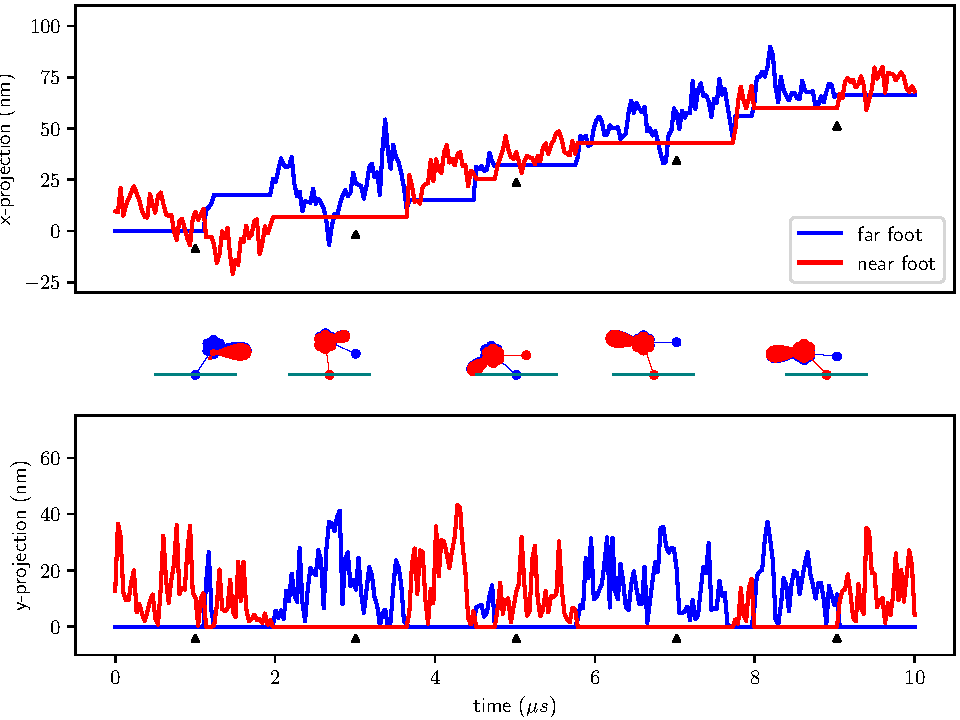
\includegraphics[width=\linewidth]{../../plots/paper_trajectory_plot.pdf}
%\caption{\textbf{Model achieves forward-directed processivity.} \textit{Top view:} x-position of near and far binding domains during a 10 $\mu s$ simulation at high kinetic parameters of $k_b = \trajectorykb s^{-1}$ and $k_{ub} = \trajectorykub s^{-1}$. \textit{Middle view:} Cartoon snapshot of model at time indicated by bound binding domain. Teal lines correspond to the microtubule. \textit{Bottom view:} y-projection. Arrows on top and bottom plots correspond to respective snapshot times.}
%\label{fig:trajectory}
%\end{figure}

The model was then compared to TIRF studies of dynein stepping in DeWitt \textit{et. al.} \cite{yildizpaper}. Figure \ref{fig:behavior}.a shows 8 representative model trajectories compared to experimental dynein. The eight simulations track experimental very well over 5 seconds, and average to the same position. The eight simulations end up distributed over a 200 \textit{nm} area, showing the variation in the model stepping extends to a variation in velocity in the long term. The step size distribution for the 32 simulations are shown in Figure \ref{fig:behavior}.b). The model is capable of taking both positive and negative steps, with steps extending from -40 \textit{nm} to 50 \textit{nm}, matching experimental dynein. The most probable step is 12 \textit{nm}, with an average step size of 6.2 \textit{nm}. This matches the peak experimental step size window of 7-13 \textit{nm}. The pre-stroke and post-stroke state occupation times are shown in Figure \ref{fig:behavior}.c and d.). The model prefers long pre-stroke times, but is capable of taking very fast steps. The post-stroke time has a heavy-tailed distribution. Experimental technique does not resolve time spent in pre- and post-stroke, but we outline a technique for calculating these values for experimental trajectories in Methods. These theoretical values correspond well to model behavior, and square with experimental findings that dynein is almost always in the post-stroke state \cite{imaiburgess}.

%\begin{figure}[tbhp]
%  \centering
%  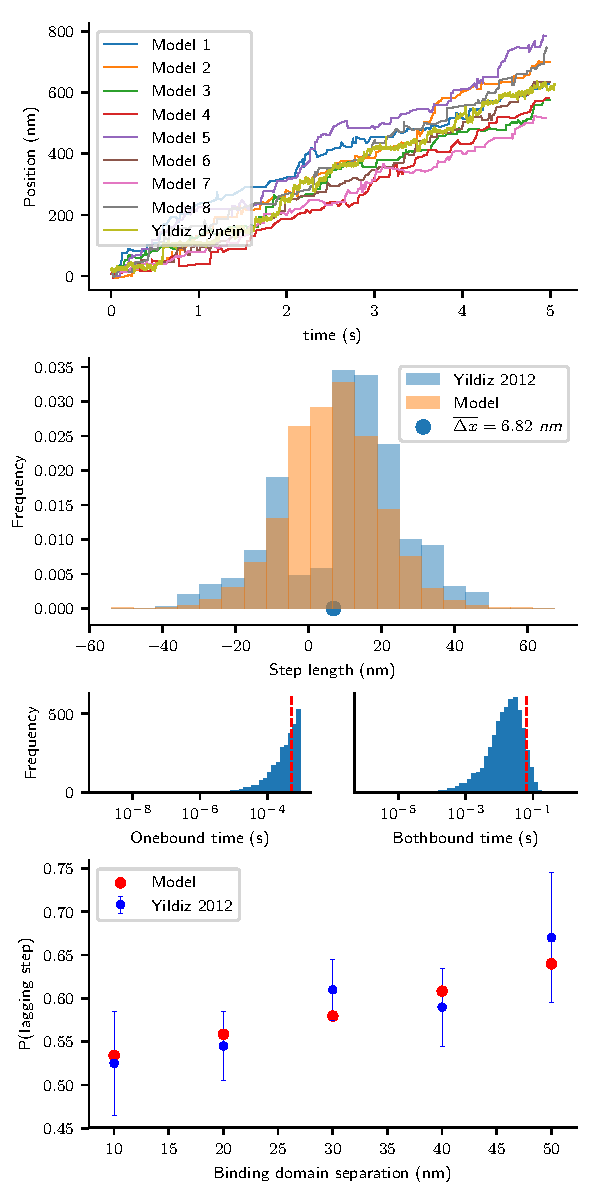
\includegraphics[width=\linewidth]{../../plots/paper_model_behavior}
%\caption{\textbf{Stepping dynamics of model.} \textit{Top: } Average position of near and far MTBDs over 5 seconds of simulation and 8 random seeds. Trajectory compared with single-motor-labelled cytoplasmic dynein from DeWitt \textit{et. al.} \cite{yildizpaper}. \textit{Middle: } Model step size distribution from 32 5 second simulations. Step length is defined as the change in an MTBD position during a full step cycle. Also plotted is the head step size distribution from DeWitt \textit{et. al.} \cite{yildizpaper}. \textit{Bottom left: } Distribution of time spent in the pre-stroke state during a full mechanochemical cycle from the same dataset. \textit{Bottom right: } Time in the post-stroke state. Both bottom plots have the theoretical values for pre-stroke and post-powerstoke times from the DeWitt \textit{et. al.} stepping trajectory.}
%\label{fig:behavior}
%\end{figure}

Dependence of the unbinding MTBD on its relation to its partner MTBD is studied in Figure \ref{fig:tensiongating}. Figure \ref{fig:tensiongating}.a shows a heat map of initial displacement, defined as how much the stepping MTBD is ahead of the stationary MTBD, vs the step size. A line of best fit is constructed with intercept $b=5.7$ and slope $m=-1$. This indicates a negative trend where large positive displacements are likely to cause backwards steps, and negative displacements are likely to cause forward steps. This is consistent with the idea of tension gating, where tension between the two motor heads drives unbinding to relieve tension. The negative trend is reproduced in DeWitt \textit{et. al}, which shows a slope of $m=-0.4$. Figure \ref{fig:tensiongating}.b shows the unbinding probability of the lagging head with distance to the leading head. As the distance becomes greater the lagging head is more and more likely to unbind, again consistent with tension gating. This trend also very closely tracks DeWitt \textit{et. al}.

%\begin{figure}[tbhp]
%  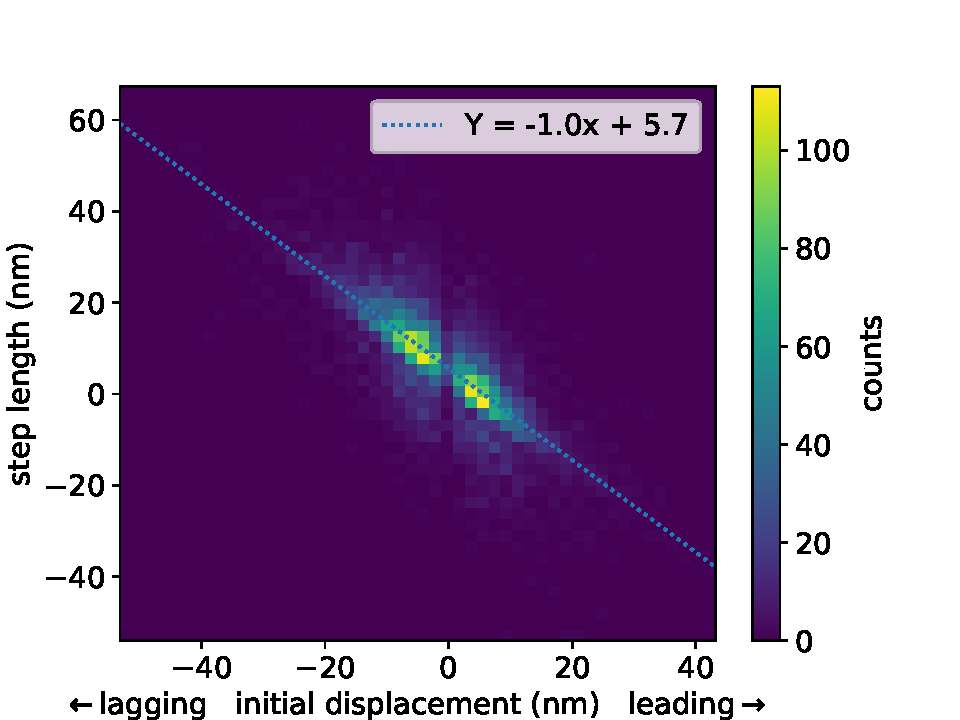
\includegraphics[width=\linewidth]{../../plots/paper_displacement_vs_step_length.pdf}
%  \includegraphics[width=\linewidth]{../../plots/paper_unbinding_probability_vs_displacement.pdf}
%  \caption{\textbf{Analysis of foot order on unbinding.} \textit{Top: } Heatmap of initial foot position vs length of ensuing step. Initial displacement defined as position of the stepping MTBD minus the position of the stationary MTBD, before the step takes place. Line of best fit calculated with equation shown in legend in orange. Line of best fit from the same plot in DeWitt \textit{et al} \cite{yildizpaper} on cytoplasmic dynein shown in blue. \textit{Bottom: } Likelihood of a lagging-MTBD unbinding event vs the absolute value of initial displacement for model. The lagging-MTBD is the MTBD with more negative x position. Probability calculated as P(lagging step)$ = k_{ub}^{\text{lag}} / \left(k_{ub}^{\text{lag}} + k_{ub}^{\text{lead}}\right)$, where $k_{ub}^{\text{lag}}$ is the lagging-MTBD unbinding rate and $k_{ub}^{\text{lead}}$ the leading-MTBD unbinding rate. Lagging step probability also shown for DeWitt \textit{et. al.} cytoplasmic dynein.}
%  \label{fig:tensiongating}
%\end{figure}

The effect of force on the model was then assessed by applying an artificial force on the tail domain of the model in the $+\hat{x}$ direction. The results of this study are shown in Figure \ref{fig:force}. An expected decrease in velocity is seen as stronger and stronger negative forces are applied to the model, pulling it against its natural walking direction. Unlike experiment, a reversal in velocity is not seen for this trial, indicating that perhaps the dynamics of force-mediated velocity reversal are more complicated than what this simplified model can handle. The results are consistent with an experiment done by Grotjahn \textit{et. al} where force is applied via optical tweezers to dynein constructs and their velocity is assayed. It will need to be studied why odd behavior is seen in the mdoel for positive forces.

%\begin{figure}[tbhp]
%  \centering
%  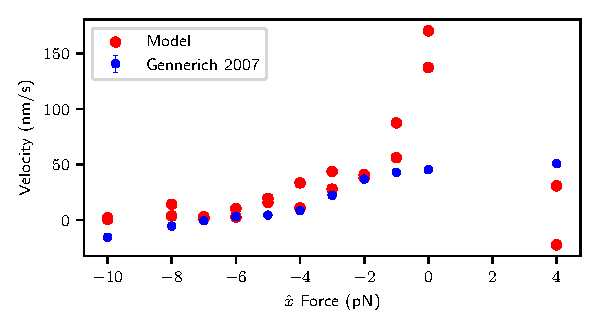
\includegraphics[width=\linewidth]{../../plots/paper_force_vs_velocity.pdf}
%\caption{\textbf{Impact of force on model velocity.} Model response to force in the $+\hat{x}$ direction applied to tail domain. Velocity calculated using displacement after 2 seconds of simulation at standard parameters. Behavior compared with a similar experiment on a cytoplasmic dynein construct using optical tweezers from Gennerich \textit{et. al.} \cite{responsetoload}.}
%\label{fig:force}
%\end{figure}

The independence of dynein steps is then studied in Figure \ref{fig:independence}. Whether dynein works like a Markovian process, where each step is a history-free, is an interesting question. Figure \ref{fig:independence} demonstrates the impact of initial displacement of MTBDs to their final displacement, before and after a step is taken. The asymmetry in the plot is indicative that the initial configuration of the motor does have significant impact on the later state. The Brownian forces act to mitigate momentum and prevent information transfer through motion. However, the binding orientation of the dynein model to the microtubule is stable through time, and can influence the binding orientation of dynein to the microtubule at a later time. There seems to be a roughly tension-gated process occurring where negative displacements initially lead to positive displacements later.

%\begin{figure}[tbhp]
%  \centering
%  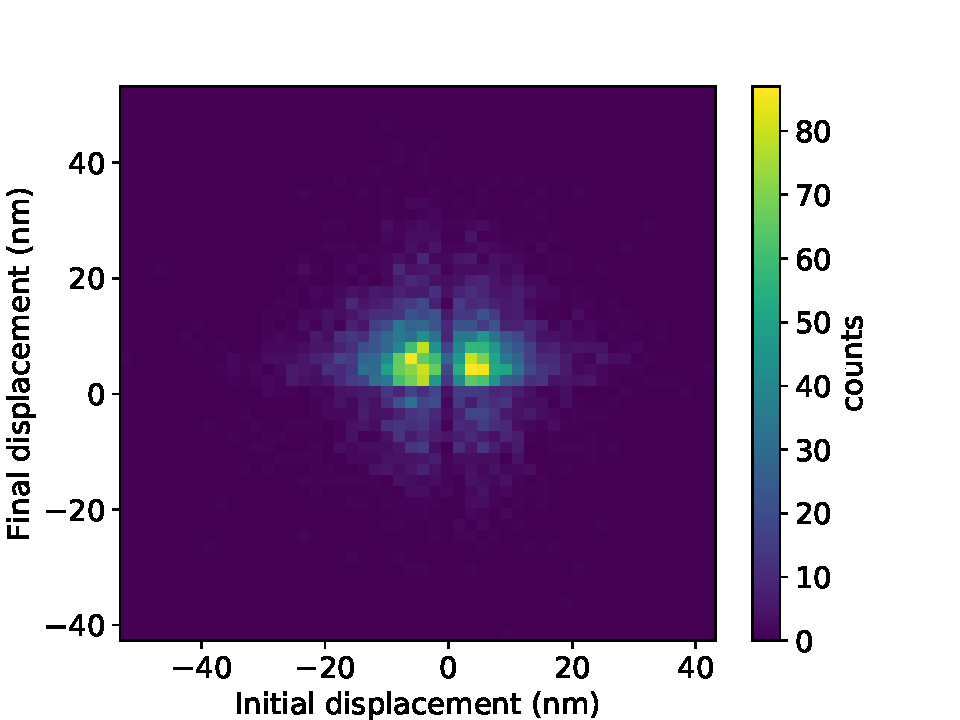
\includegraphics[width=\linewidth]{../../plots/paper_initial_vs_final_displacement.pdf}\\
%  \includegraphics[width=\linewidth]{../../plots/paper_stacked_displacement_histogram.pdf}
%  \caption{\textbf{Analysis of stepping independence.} \textbf{a.)} Heatmap of MTBD displacement before and after a stepping cycle. Displacement defined as the unbinding MTBD's x coordinate minus the stationary MTBD's x coordinate, calculated before and after the step. Structure in the heat map suggests steps are not independent, but rather that correlation exists between starting position and step size. \textbf{b.)} Compound histogram of final displacement for different ranges of initial displacement.}
%\label{fig:independence}
%\end{figure}

%\begin{figure}[tbhp]
%  \centering
%  \begin{subfigure}[]{0.8\columnwidth}\caption{}\vspace{5pt}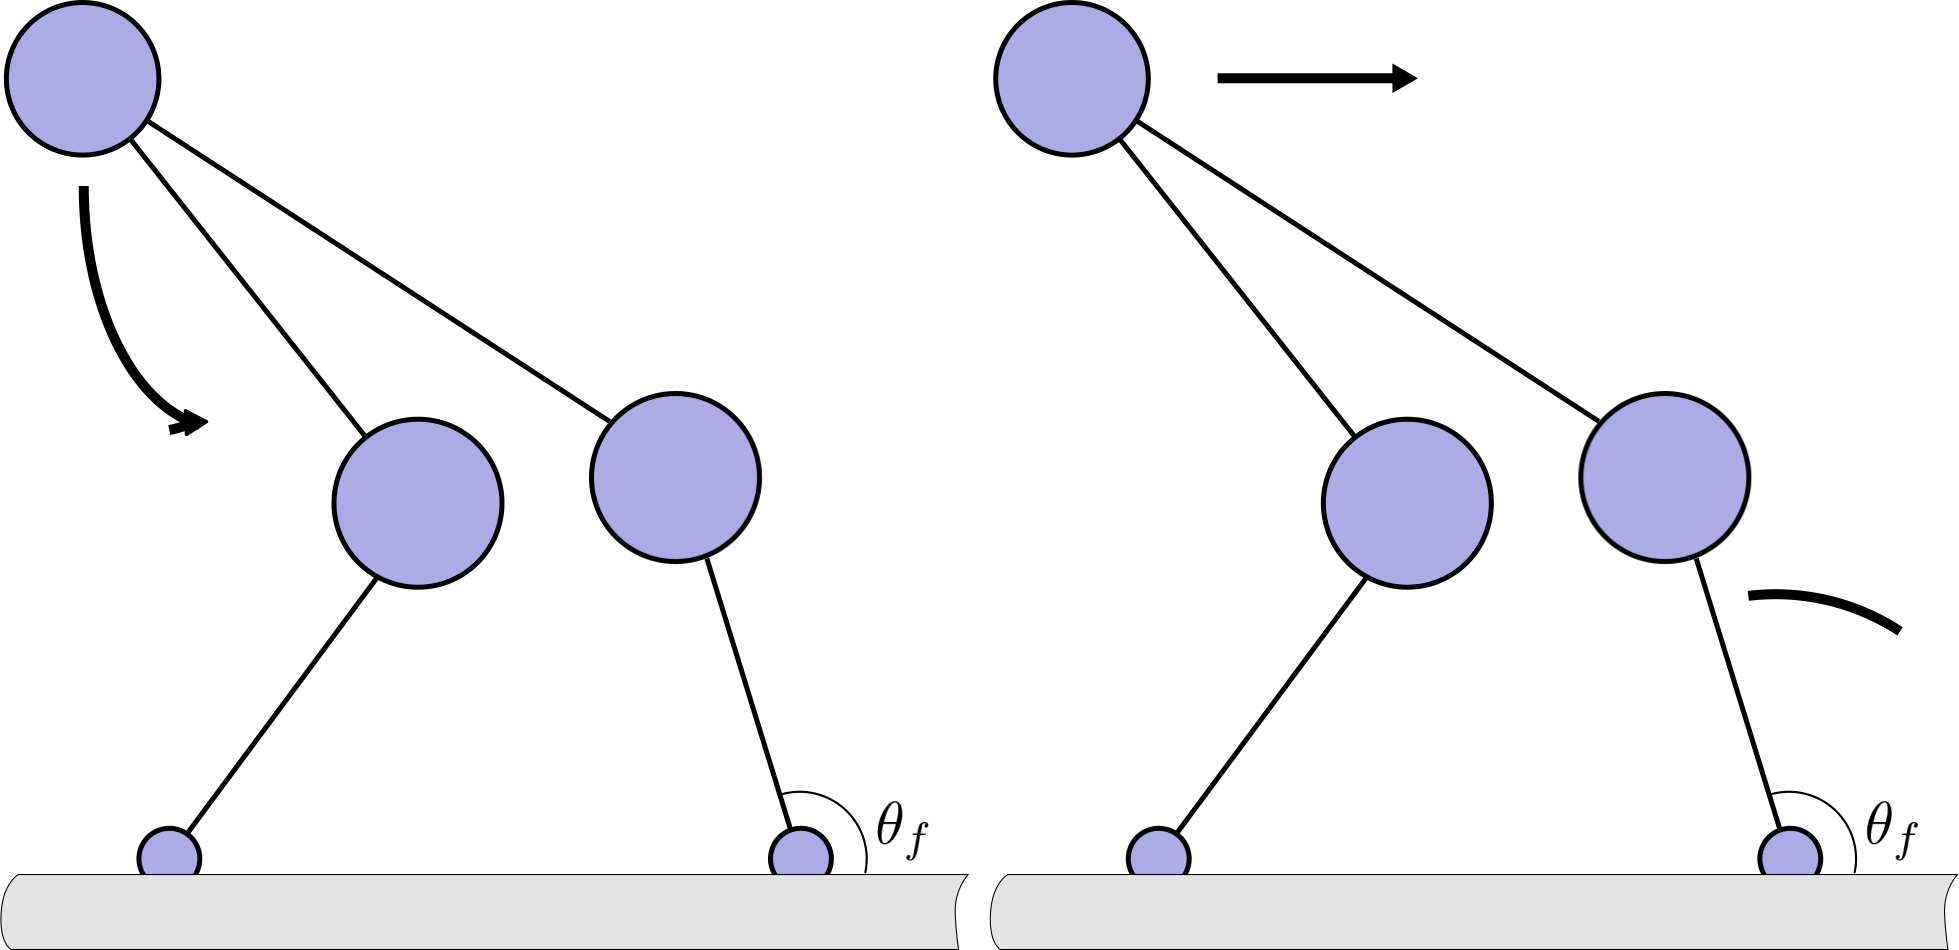
\includegraphics[width=\columnwidth]{figures/winch-powerstroke-cartoon}\end{subfigure}\vspace{10pt}\\
%  \begin{subfigure}[]{0.5\columnwidth}\caption{}\includegraphics[width=\columnwidth]{../../plots/bothbound_stroke_angles_bd}\end{subfigure}%
%  \begin{subfigure}[]{0.5\columnwidth}\caption{}\includegraphics[width=\columnwidth]{../../plots/bothbound_stroke_angles_md}\end{subfigure}\\
%  \begin{subfigure}[]{0.5\columnwidth}\caption{}\includegraphics[width=\columnwidth]{../../plots/bothbound_stroke_tailx_positions}\end{subfigure}%
%  \begin{subfigure}[]{0.5\columnwidth}\caption{}\includegraphics[width=\columnwidth]{../../plots/bothbound_stroke_taily_positions}\end{subfigure}\\
%  \begin{subfigure}[]{0.5\columnwidth}\caption{}\includegraphics[width=\columnwidth]{../../plots/bothbound_long_stroke_angles_bd}\end{subfigure}
%  \caption{\textbf{Dynein model exhibits powerstroke, not winch, dynamics.} \textit{A. left: } Schematic of winch model for dynamics during conformation changes associated with right monomer binding. On free MTBD binding, linker swing in the just-bound head pulls the tail and cargo in the direction of the just-bound MTBD. \textit{A. right: } Schematic of the powerstroke model for dynamics during during conformation changes associated with right monomer binding. On free MTBD binding, linker swing pushes the just-bound head and tail domains towards the minus-end of the MT and alters the just-bound stalk domain's angle with the MT. Subfigures b-e describe dynamics for the right monomer during post-binding conformation change; only data for steps with a positive step size is shown. \textit{b.) } Just-bound MTBD stalk angle relative to MT axis as a function of time since MTBD binding along with MTBD angle equilibrium (blue dotted line). \textit{c.) } Just-bound head angle, along with prestroke equilibrium (red dotted line) and poststroke equilibrium (blue dotted line). \textit{d.) } Change in tail domain x coordinate since MTBD binding. \textit{e.) } Value of tail domain y coordinate. All values sampled every $10 ns$. \textit{f.) } Just-bound MTBD stalk angle for the millisecond after binding, sampled every 20 $\mu s$. All values plotted as mean $\pm$ SD.}
%\label{fig:stroke}
%\end{figure}

We then examined how the model took its forward steps. Two existing theories for motion generation are depicted in Figure \ref{fig:stroke}.a. The winch model \cite{carterwinch, uenoem, sarlahmodel, nicastro, kinoshitaPSwinch, lippert}, on the left, predicts that the prestroke to poststroke transition causes the just-bound motor's head to act like a winch, pulling the tail domain down and forwards toward the microtubule. The powerstroke model \cite{mallikps, burgessknight, robertspowerstroke, burgess-paper}, on the right, predicts that the transition will cause a lever-like action of the just bound stalk, pulling the just bound motor's head and tail forward. The most notable differences between these two models are whether the stalk angle changes during the stroke \cite{lippert}, and whether the tail domain moves closer or further from the microtubule. Arrows indicate these predictions in Figure \ref{fig:stroke}.a.

The average change of motor angles and positions during the prestroke-to-poststroke transition is shown in subfigures \ref{fig:stroke}.b-e. Only positive steps were used for clarity. Subfigure \ref{fig:stroke}.b indicates the model's just-bound stalk experiences a consistent angular displacement after binding, rotating to point more towards the minus end of the MT. Interestingly, this transition takes the binding angle out of equilibrium. This transition is permanent once made, as shown in \ref{fig:stroke}.f, which shows the no change even up to a millisecond after binding. This forward transition of the head domain is accompanied by a forward displacement of the tail domain by roughly 12 $nm$, as shown in Figure \ref{fig:stroke}.d, and a displacement away from the microtubule by 5-8 $nm$, as shown in Figure \ref{fig:stroke}.e. This tail displacement takes roughly 300ns, which corresponds roughly to the prestroke-to-powerstroke transition time from MD \cite{mdstroke} (DOES IT ACTUALLY THOUGH? LOOK AGAIN). The motor angle is shown in Figure \ref{fig:stroke}.c to transition from the pre-stroke equilibrium to the post-stroke equilibrium in time with the stalk angle change. Taken together, this data indicates that our simulated dynein moves through a powerstroke-, not a winch-type mechanism. We hypothesize that the out of equilibrium state of the motor angle post-transition is highly energetic, and it is quicker for the model to re-equilibrate the high-energy state through pushing the motor forward in a powerstroke than winching the faraway bulky tail downwards.

%% \begin{figure*}[tbhp]
%%     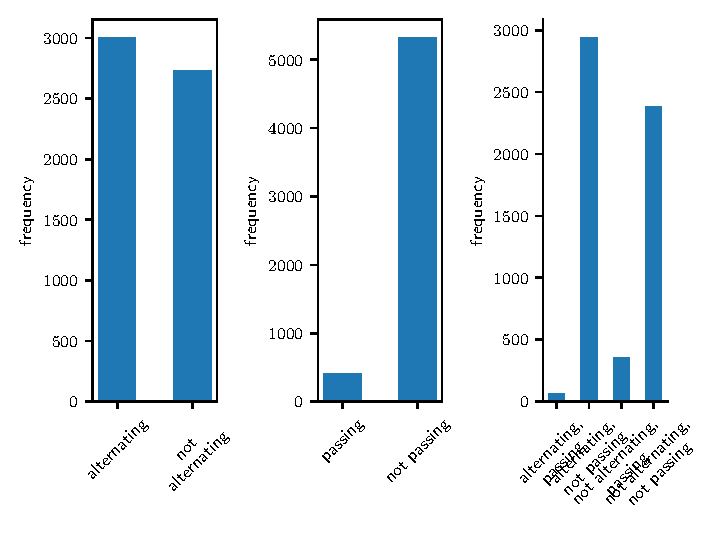
\includegraphics[width=0.5\linewidth]{../../plots/paper_foot_order_histogram.pdf}
%% \caption{The left plot is the $C=0$ case where the unbinding rate is
%%   independent of angle.  Here ``alternating'' means that the binding
%%   domain which did not move last time moved this time.  Passing means
%%   that the moving foot was behind, and ended up in front.}
%% \label{fig:steppingorder}
%% \end{figure*}

\section{Discussion}
In this study we sought to study dynein's dynamics using a simple model. We used imaging data to construct a structurally realistic goemetric model for the motor, then used Brownian dynamics to explore how such a model would behave in a cell. We used experimental data on dynein's step length distribution and unbinding likelihood to fit the model's spring and tension-gating constants. We used arguments about dynein's run length and velocity to predict the average time the motor spent in the pre-stroke and post-stroke states, and fit the model's binding and unbinding rates to these predictions. From fitting we found that relatively loose tail and MTBD spring constants and a stiff motor domain produced the best stepping histogram; this agrees with another simulation which found tail and MTBD flexibility is necessary for large steps \cite{tsygankovemsimulation}. We tested the dynamics of this fit model, and found that the model displayed a high level of agreement with the data used to fit; the simulation's velocity and stepping histogram in Figure \ref{fig:behavior} match experiment quite well. In addition the model can predict new data it was not fit with, such as force output in Figure \ref{fig:force} and effects of foot displacement on step length in Figure \ref{fig:tensiongating}. The model also displays both inchworm and hand-over-hand stepping, as in real dynein \cite{weihongpaper}. The ability of our model to replicate basic experimental features indicates that the core of dynein's step is its ability to couple conformational transitions with MT affinity, and no other aspects are needed. The major deviation in model and experiment is the step length density of model steps around 0nm, which is possibly caused by an inability of the step detection algorithm to detect small steps in experimental dynein. We then examined the mechanism our model used to walk by studying domain positions over many steps. We found that the majority of forward displacement occured immediately after a free binding domain bound to the microtubule, when the just-bound stalk swung forward, pulling the attached motor and tail domains toward the minus-end of the microtubule.

One of the main advantages of our study is that it makes predictions with high spatial and temporal resolution using dynamics realistic for a protein of dynein's size and environment. This allows us to study mechanistic questions about how dynein walks, which has not been done before. Interestingly, our minimal model, with no assumptions about the dynamics of dynein's forward step, appears to generate motion using the powerstroke mechanism long-theorized to account for dynein's motion \cite{mallikps, burgessknight, robertspowerstroke, burgess-paper}. As our model transitions from the so-called pre-stroke to post-stroke state it increases its head angular spring energy from a shifting motor equilibrium angle; it relaxes this high motor energy by rotating its stalk towards the minus-end of the MT, pulling the motor and tail domains with it. This increase in head spring energy is roughly analogous to the high-energy state of the head of real dynein after MTBD binding induces Pi rejection and linker swing \cite{MANY-CITATIONS-HERE}. The stalk angle remains displaced from equilibrium until the next unbinding. Our simulations support the idea that a powerstroke-like mechanism also occurs in real dynein, where angular displacement of the just-bound stalk pulls the motor and tail domains forward. The fact that our model only assumes a harmonic restoring energy and a transition in equilibrium angles when switching states, yet produces a robust powerstroke, supports the idea that the powerstroke is feasible for a protein of dynein's general shape and size. The fact that a winch-like mechanism was not the dominant mechanism may indicate that the winch is more infeasible for a dynein-like protein. This may be due to the fact that the winch requires dragging a potentially large tail domain, whereas the powerstroke only requires pushing the motor domain forward. (Not sure if this makes sense, re-check).

This model contrasts with another theory on the dynein step called the winch mechanism \cite{carterwinch, uenoem, sarlahmodel, nicastro, kinoshitaPSwinch, lippert} (note: literature uses the term ``winch'' in different ways; we use the definitions from \textit{Lippert et. al} \cite{lippert}). According to this model, on MTBD rebinding, linker swing puts the just-bound head in a high energy state, just like in the powerstroke mdoel. However, to relieve this tension the motor instead ``winches'' its tail domain downwards in the direction of the stalk, resulting in a tail which is closer to the MT and further forward. To our knowledge, no previous simulation has tested the physical feasibility of either the winch or powerstroke models. Although our model is a minimal depiction which does not take into account the acute dynamics of the whole motor, its ability to reproduce the dynamics of the real dynein suggests that it may have some bearing on how the real dynein walks. In particular, this model spontaneously exhibits the powerstroke mechanism, suggesting that the powerstroke mechanism is both feasible for the dynein complex to generate and sufficient to explain much experimental data. Although this does not rule out the winch mechanism as an explanation, we believe that the lack of any winch-like behavior in our simulation is meaningful. Indeed during displacement our model's tail domain actually moves away from the microtubule, the opposite of the winch's prediction. Further theoretical studies demonstrating the feasibility and sufficiency of the winch mechanism are needed.

Recent experimental studies have had strong implications for the winch vs powerstroke mechanisms. A key question is whether the just-bound stalk experiences angular displacement as the motor moves forward, as this is necessary for the powerstroke and not the winch. This angular displacement was not found by Lippert \textit{et. al.} \cite{lippert}, who used polTIRF to study the angle dynein's stalk made with the MT in freely-walking dynein. Another study showed that there is no difference in stalk angle between motors locked in the pre- and post-stroke state using special nucleotides and cryo-electron microscopy \cite{uenoem}. One key finding of our study which reconciles the powerstroke mechanism with these experimental findings is the timescale on which the predicted stalk angular displacement occurs. We find that the average duration of the angular displacement period of the just-bound stalk is on the order of 1 $ms s$ from the prestroke diffusive search, as the actual angular displacement during the powerstroke is negligibly small (see Figure \ref{fig:stroke}). According to the powerstroke model the stalk should be displaced after the recovery stroke, during ATP hydrolysis and Pi release, after binding the MT, and during the powerstroke, in the most likely progression through the mechanochemical cycle \cite{tsygankovscheme}. Our calculations for the time only one head is bound predict this period to last roughly 1 $ms$. Thus, assuming the MT-bound prestroke period is short enough \cite{mogamirate}, it is possible the entire displacement period should be on the order of milliseconds. This time could be faster than the 50 $ms$ time resolution of the polTIRF experiment of Lippert \textit{et. al.}, which may explain why an angular displacement was not detected. Furthermore we note that in our model the stalk angle deviates from equilibrium as the motor and tail move forwards; only much later does the stalk return to equilibrium. This suggests that the stalk angular displacement is a non-equilibrium phenomena which could not be detected through cryo-EM, which resolves equilibrium structures. This explains why cryo-EM studies have not been able to find the angular displacement \cite{uenoem, nicastro} (REREAD THE UENOEM PAPER TO MAKE SURE THIS IS RIGHT). We further hypothesize that previous simulation results \cite{sarlahmodel}, which have shown a winch-like mechanism is capable of generating motion, have only done so because they do not account for drag and diffusion dynamics. Our data demonstrate that pushing forward the motor domain in a powerstroke is a more likely means of relieving the high-energy poststroke state than winching down the far off tail. We hypothesize that further models which also account for diffusion would find the same. We suggest that the powerstroke mechanism has not been disproven by these studies, and that in order to show the powerstroke doesn't exist, an experiment must be done with high enough time-resolution to resolve the fast microsecond phenomena.

Our study demonstrates other interesting findings. Similar to past simulation work \cite{sarlahmodel}, we demonstrate that our model is capable of achieving minus-end directed motility merely through the way it binds to the microtubule. Also interestingly, we demonstrate that our model is capable of taking 12$nm$ (CHANGE ON RERUN) steps in the absence of explicit microtubule binding sites. Merely through the size of its stalk and tail and through the magnitude of angular displacement induced by linker swing, our model is capable of taking the right step size. It is interesting that in our model a single step is slightly shorter than the experimental 16nm step \cite{find-citation}. This suggests that perhaps the motor requires a diffusive search along the microtubule to find the next binding site. Alternatively, as has been recently demonstrated, perhaps an electrostatic mechanism is used to guide the MTBD to the next binding site using long-range interactions \cite{longrangemt}.

Our theoretical work draws upon and extends several past models \cite{sarlahmodel, trottmodel, tsygankovemsimulation, zhaomodel}. This paper's approach of using Brownian dynamics to realistically predict the diffusion dynamics of a structural model of dynein is a useful technique for testing mechanistic theories for biological feasibility and sufficiency, and to our knowledge is the first model to combine imaging and kinetics data with Brownian dynamics to quantify the influences of drag on the dynein motor. We believe that taking into account diffusion dynamics and drag is necessary to understand dynein's dynamics, and not doing so may explain why previous studies found the winch model to replicate experimental results \cite{sarlahmodel}. Our minimal assumptions simplify the model and allow analytical solutions to motion equations. However, our model neglects many features which may be important for real dynein's walk. For example, some have proposed that stalk flexibility is an important aspect of dynein's mechanism \cite{mdstalk, lippert, find-that-other-possibly-burgess-paper}. Other features like microtubule electrostatic interactions \cite{longrangemt}, binding angle dependent MTBD binding \cite{responsetoload} - ACTUALLY LOOK AT PAPER THOUGH, inter-head coordination \cite{tsygankovscheme, tsygankovemsimulation}, stalk flexibility???, Y and Z are also neglected. Although our work successfully demonstrates the sufficiency of our minimal set of assumptions for generating motion, a more biologically realistic model would need to take these listed features into account.

In conclusion, our study demonstrates that the powerstroke mechanism is sufficient to explain dynein's velocity, step length histogram, displacement-vs-step length relationship, and force output. We demonstrate that the powerstroke arises naturally from minimal structural information about the protein, suggesting it is likely possible for real dynein to exhibit a powerstroke. Further, we explain why past studies may have failed to detect this powerstroke. We hope that this evidence is sufficient to maintain the powerstroke mechanism as a viable hypothesis for how dynein walks. We further hope that experiments with higher spatial and temporal resolution can be conducted in the near future to shed more light on the precise nature of dynein's stepping mechanism.

\section{Papers we should cite}
This paper says something interesting~\cite{leschziner}.

\bibliographystyle{unsrt}
\bibliography{paper}

\end{document}
